\documentclass[conference,10pt]{IEEEtran}

\usepackage{url}
\usepackage{amsmath}
\usepackage{amssymb}
\usepackage{zed-cm}
\usepackage{graphicx}
\usepackage{dblfloatfix}

%\renewcommand \thefigure{\Roman{figure}}

\begin{document}

\title{PODD - Towards An Extensible, Domain-agnostic Scientific Data Management System}

\author{\IEEEauthorblockN{Yuan-Fang Li, Gavin Kennedy, Faith Davies and Jane Hunter}
\IEEEauthorblockA{School of ITEE, The University of Queensland\\
Brisbane, Australia\\
Email: \{uqyli4,g.kennedy1,f.davies,j.hunter\}@uq.edu.au}
}

\maketitle


\begin{abstract}
Data management has become a critical challenge faced by a wide array of scientific disciplines in which the provision of sound data management is pivotal to the achievements and impact of research projects. Massive and rapidly expanding amounts of data combined with data models that evolve over time contribute to making data management an increasingly challenging task that warrants a rethinking of its design. In this paper we present PODD, an ontology-centric architecture for data management systems that is extensible and domain independent. In this architecture, the behaviors of domain concepts and objects are captured entirely by ontological entities, around which all data management tasks are carried out. The open and semantic nature of ontology languages also makes PODD amenable to greater data reuse and interoperability. To evaluate the PODD architecture, we have applied it to the challenge of managing phenomics data. 
\end{abstract}

\begin{IEEEkeywords}
PODD, data management systems, OWL, ontology-centric architecture, phenomics
\end{IEEEkeywords}

\section{Introduction}\label{sec:intro}
Data management is the practice of managing (digital) data and resources, encompassing a wide range of activities including acquisition, storage, retrieval, discovery, access control, publication, integration, curation and archival. For many data-intensive scientific disciplines such as life sciences and bioinformatics, sound data management informs and enables research and has become an indispensable component~\cite{1107503}.

The need for effective data management is, in a large part, due to the fact that massive amounts of digital data are being generated by modern instruments. Furthermore, the fast evolution of technologies/processes and discovery of new scientific knowledge require flexibility in handling dynamic data and models in data management systems. Among others, there are three core challenges for effective data management in scientific research.

\begin{itemize}
\item The ability to provide a data management service that can manage large quantities of heterogeneous data in multiple formats (text, image, and video) and not be constrained to a finite set of experimental, imaging and measurement platforms or data formats.

\item The ability to support metadata-related services to provide context and structure for data within the data management service to facilitate effective search, query and dissemination.

\item The ability to accommodate evolving and emerging knowledge, technologies and processes.
\end{itemize}

Database systems have traditionally been used successfully to manage research data~\cite{brm2007} in which database schemas are used as domain models to capture attributes and relationships of domain concepts. One implication of the above approach is that domain models need to stay relatively stable as database extension and migration is often an error-prone and laborious task. Consequently, this approach is not suitable for domains where data and model evolution is the norm rather than the exception.

Semantic Web ontology languages such as RDF Schema and OWL possess expressive, rigorously-defined semantics and non-ambiguous syntaxes. Moreover, they have been designed to be open and extensible and to support knowledge and data exchange on the Web scale~\cite{linkeddata,aue07dbpedia}. These intrinsic characteristics make them an ideal conceptual platform on which a flexible scientific data management system can be built.

Ontology language OWL has been widely used in a number of domains, notably in life sciences and biotechnology~\cite{journals/bib/RuttenbergRSM09,citeulike:1882392,citeulike:212874} as a modeling language for its expressivity and extensibility. There is also growing tool support for tasks including reasoning, querying and visualization, making it a viable option for the modeling and representation of scientific domain concepts.

Moreover, with the rapid progression of Semantic Web-based data integration through the community-driven Linked Data project~\cite{citeulike:5008761}, it is advantageous for data management systems to support Semantic Web languages and standards natively to benefit from the rapidly expanding, integrated open datasets. 

In this paper, we present our work in designing PODD (Phenomics Ontology Driven Data Management), an extensible, domain-agnostic architecture for scientific data management that uses an ontology-centric approach. In our architecture, we support data and model changes through ontology-based domain modeling. Ontologies are at the core of the system - the behaviors of abstract domain concepts and concrete domain objects are entirely defined by ontological vocabularies. Logical structure of data is therefore maintained and enforced via ontological definitions and reasoning and not via database schemas and associated constraints. 

The ontology-based domain model is at the core of PODD as it drives the creation, storage, validation, query and search of data and metadata. In contrast to traditional data management systems that use database schemas as the underlying model, the layered object-oriented approach to developing ontology models and the versioning of ontological definitions make PODD highly extensible. 

Based on the ontology-centric architecture, we have developed the PODD repository~\cite{podd_icadl} to meet the above challenges facing the Australian phenomics research community. Our aim is to provide efficient and flexible repository functionalities for large-scale phenomics data, and to provide a mechanism for maintaining structured and precise metadata around the raw data so that they can be stored, distributed and published in a reusable fashion. 

We would like to emphasize that although the PODD system is geared towards phenomics research, the ontology-centric architecture we propose in this paper is domain-independent and can be applied in any scientific discipline where research output can be conceptually organized in a structured manner. 

The rest of the paper is organized as follows. In Section~\ref{sec:overview} we present related work and give a brief overview of the motivation and goals of the PODD project. Section~\ref{sec:arch} presents the ontology-based architecture for data management systems. In Section~\ref{sec:ont}, we discuss the PODD ontologies in more detail and show how the ontology-based modeling approach is used in the life cycle of repository concepts and objects. In Section~\ref{sec:sys}, we describe the implementation of the PODD data management system and evaluation results to date. Finally, Section~\ref{sec:concl} concludes the paper and identifies future directions.

\section{Related Work, Motivation \& Goals}\label{sec:overview}
Over the years attempts have been made to develop content repository systems and architectures to meet institutional and personal data management needs. In this section, we introduce a number of such systems and architectures. With a survey of related work, we present the motivation behind the ontology-centric architecture and the goals we wish to achieve with the PODD data management system.

\subsection{Scientific Data and Resource Management Systems}
A number of open-source content repository specifications and scientific data management systems have been developed.

Fedora Commons\footnote{\url{http://www.fedora-commons.org/}} is an open-source digital resource management system based on the principles of modularity, interoperability and extensibility. In Fedora Commons, abstract concepts are defined as models, on which inter-relationships and behaviors can be further defined. Data in Fedora Commons repositories are represented as objects, which contain datastreams that store either metadata or data. Fedora Commons makes heavy use of Semantic Web technologies through the use of common RDF vocabularies and the integration with the Mulgara triple store\footnote{\url{http://www.mulgara.org/}}, which can be used for metadata storage and query through SPARQL. 

Apache Jackrabbit\footnote{\url{http://jackrabbit.apache.org/}} is an open-source implementation of the Content Repository for Java Technology (JCR) API\footnote{\url{http://jcp.org/en/jsr/detail?id=283}}. In JCR, data is stored in a tree of nodes, which can hold properties of arbitrary values, which is conceptually similar to Fedora Commons. Types can be defined on nodes to place certain restrictions on them.

Fedora Commons and JCR both support fairly basic mechanisms for defining object relationships. Hence, they are usually used as the underlying repository solution on which complex data and document management systems are built. These systems include the National Science Digital Library (NSDL)\footnote{\url{http://nsdl.org/}}, PLoS ONE\footnote{\url{http://www.plosone.org/}}, Biodiversity Heritage Library\footnote{\url{http://www.biodiversitylibrary.org/}} and Fez\footnote{\url{http://fez.library.uq.edu.au/}}, among others. As stated previously, these systems use database schemas as their domain models.

Data management systems have also been developed to support a number of scientific disciplines including high-energy physics, bioinformatics and Earth observation~\cite{652836}.

Bioinformatics Resource Manager (BRM)~\cite{brm2007} is one example of client-server style data management software for bioinformatics research. The client software is installed on users' computers to access (microarray and proteomic) resources stored on BRM server in a PostgreSQL relational database. The BRM server supports data acquisition from external sources such as NCBI~\cite{ncbi} and UniProt~\cite{citeulike:503151}. It also supports annotation using public datasets and connectivity to analytics tools. Data in BRM is stored under the \emph{Project} concept and is mostly flat, i.e., it does not support hierarchical domain concepts such as investigation and publication. SciPort~\cite{1326001} is a peer-to-peer based platform for scientific data integration.

Besides data management systems, grid-based middleware systems have also been developed to provide distributed storage solutions. Such systems include the Storage Resource Broker (SRB)~\cite{783165} and the CERN Data Grid~\cite{652836} and other systems that make use of Globus\footnote{\url{http://www.globus.org/}} middleware. These systems store data in a distributed environment and usually support authentication, replication, redundancy, etc. However, they are mostly only concerned about data storage and replication and hence do not provide full-fledged data management capabilities. Interested readers are referred to~\cite{565296} for a detailed survey of grid resource management systems. Semantic Grid\footnote{\url{http://www.semanticgrid.org/}} is an extension of Grid technology in which rich metadata is made available to and managed explicitly by applications in the grid. A reference architecture for semantic grid, S-OGSA~\cite{citeulike:1021910}, has been proposed that defines a model and capabilities and mechanisms for the Semantic Grid.

More recently, ontology-based approaches have been taken in VIVO~\cite{vivo10} to model, organize and integrate research activities and researcher profile in an institutional setting.

\subsection{Domain Modeling in Scientific Research}
A number of specifications and ontologies have been proposed to model scientific research activities. In 2004, Council for the Central Laboratory of the Research Councils (CCLRC) of UK developed a CCLRC Scientific Metadata Model~\cite{Spallation_metadatamodel} that models scientific activities in free text. An OWL ontology, EXPO, was developed~\cite{citeulike:3735746} to capture metadata about scientific experiments. EXPO was developed in a top-down manner by extending concepts in the Suggested Upper Merged Ontology (SUMO)\footnote{\url{http://www.ontologyportal.org/}}. Although very comprehensive, these models are fairly verbose and not very suitable as models for developing data management systems.

In biological and particularly 'omics research, a large number of databases have been developed to host a variety of information such as genes (Ensembl\footnote{\url{http://www.ensembl.org/}}), proteins (UniProt\footnote{\url{http://www.uniprot.org/}}), publications (PubMed\footnote{\url{http://www.ncbi.nlm.nih.gov/pubmed/}}) and microarray (GEO\footnote{\url{http://www.ncbi.nlm.nih.gov/geo/}}). These databases are generally characterized by the fact that they specialize in a particular kind of data (protein sequences, publications, etc.) and that their conceptual domain models, such as genes~\cite{citeulike:212874} and microarray experiments~\cite{citeulike:151946}, are well understood.

For a scientific data management system to be effective, models of domain concepts need to be integrated with models of scientific activities and workflows. However, models of biological and clinical investigations are less well understood.

The Ontology for Biomedical Investigations (OBI)\footnote{\url{http://purl.obolibrary.org/obo/obi}} is an ongoing effort aimed at developing an integrative ontology for biological and clinical investigations. It takes a top-down approach by reusing high-level, abstract concepts from other ontologies. OBI includes 2,600+ OWL classes and 10,000+ axioms (in the import closure of the OBI ontology). Although OBI is very comprehensive, its size and complexity makes reasoning and querying of OBI-based ontologies and RDF graphs computationally expensive and time consuming, making it impractical as a domain model for data management systems where such reasoning may need to be performed repeatedly.

Functional Genomics Experiment Model (FuGe)~\cite{citeulike:1756058} is an extensible modeling framework for high-throughput functional genomics experiments, aimed at improving the consistency and efficiency of experimental data modeling for the molecular biology research community. Centered around the concept of experiments, it encompasses domain concepts such as \emph{Protocol}, \emph{Sample} and \emph{Data}. FuGe is developed using UML from which XML Schemas and database definitions are derived. The FuGe model not only covers concepts specific to scientific research such as \emph{Analysis}, \emph{Sequence} and \emph{Investigation}; it also defines commonly used concepts such as \emph{Audit}, \emph{Reference} and \emph{Measurement}. Extensions in FuGe are defined through inheritance of UML classes.

We feel that the extensibility we require is not met by FuGe as any addition of new concepts would require amendment of database schemas and code. Moreover, the concrete objects reside in relational databases, making subsequent integration and dissemination more difficult.

\vspace{-8pt}
\subsection{The PODD Repository - Motivation \& Goals}
Phenomics is a fast-growing, data-intensive discipline with new technologies and processes rapidly emerging and evolving. As a result, its domain model and data management systems must also be able to evolve to handle the complexity, dynamics and scale of the data.

In phenomics, data is usually captured by both high- and low-throughput phenotyping devices. The scale of measurement can be from the micro or cellular level, through the level of a single organism, and up to the macro or field level. Imaging, measurement and analysis of organisms on such a large scale will produce an enormous amount of data. 

Phenomics research makes use of a large variety of imaging and measurement platforms. For example, in mouse histopathology and organ pathology research, the Zeiss ``Mirax Scan'' scanner is used to scan microscope slides. In clinical pathology, a Flow Cytometer is used to capture laser diffraction images of blood samples. In plant research, the Lemnatec Scanalyzer is used to capture RGB images of plants in growth cabinets. The Fluorogroscan system is used in quenching analysis: the partitioning of light energy used in photosynthesis on model plants such as Arabidopsis. Other devices, such as the Infrared Thermography Camera are used to capture leaf temperature and the SPAD Meter is used to measure the chlorophyll content of plant leaves. New devices and instruments will also be employed as they become available. Moreover, existing instruments may be upgraded so that they can capture more information. The PODD domain model needs to be flexible to accommodate these continual changes in formats, resolution and source of the data. 

Because an organism's phenotype is often the product of the organism's genetic makeup, its development stage, disease conditions and its environment, any measurement made against an organism needs to be recorded in the context of these other metadata. Consequently the opportunity exists to create a repository to record the data, the contextual data (metadata) and data classifiers in the form of ontological or structured vocabulary terms. The structured nature of this repository will support both manual and autonomous data discovery as well as provide the infrastructure for data based collaborations with domestic and international research institutions. Currently there are no such integrated systems available. The goals of PODD are to capture, manage, annotate and distribute the data generated by mouse and plant phenomics research activities. Note that currently PODD is designed to be a data management system, it doesn't model scientific workflows.

%\vspace{-6pt}
\section{The Architecture of the Ontology-centric Data Management System}\label{sec:arch}

%\vspace{+4pt}
\subsection{Requirements of Data Management Systems}

For any scientific data management system, a number of requirements need to be satisfied.

\begin{list}{\labelitemi}{\leftmargin=1em}
\item[\textbf{Data storage and management}] Research activities in data-intensive discipline such as 'omics often generate huge amounts of data. The ability to efficiently acquire, store and manage large volumes of data is essential.

\item[\textbf{Data contextualization}] Sufficient contextual information needs to be maintained for more effective organization, understanding and discovery of raw data. Contextual information includes both conceptual domain models, such as how research activities are organized and carried out; and metadata such as provenance information.

\item[\textbf{Data security}] There are many dimensions to data security, including access control and archival. An effective data management system needs to ensure data security through the use of authentication and authorization and sound versioning and backup solutions. 

\item[\textbf{Data identification and longevity}] In order to support the dissemination of scientific findings, data in the repository needs to be publicly accessible after being published. Hence, a persistent and unique naming scheme is required. Moreover, valuable scientific data also need to be stored in perpetuity.

\item[\textbf{Data reuse and integration}] Contextual information helps to make sense of raw data. Moreover, it also needs to be made discoverable, through mechanisms such as full-text search, faceted browsing and complex query answering, to allow raw data to be integrated and reused.

\item[\textbf{Model extensibility}] A data management system may need to manage a wide variety of data, which may be generated by different software and captured by different platforms. An expressive and extensible domain model is therefore essential to cater for modification, addition and deletion of domain concepts. The data management system also needs to be designed to minimize service disruption when such a model change occurs.
\end{list}

\subsection{The PODD Ontology-centric Architecture For Data Management Systems}
The most distinguishing characteristic of PODD is the central role that ontologies play. In this architecture, raw data is not stored in a flat structure but is attached to domain objects organized in a logical, hierarchical system, defined according to the domain model that represents the structure of research activities.

Current document management systems such as Fez typically define a relatively static domain model and hardwire it as relational schemas and foreign key constraints in a custom relational database independent from the underlying repository system. Consequently, the information pertinent to each concrete object is stored in this custom database as well. As stated in the previous section, this approach is unsuitable for dynamic environments where conceptual changes are common.

To effectively support a dynamic conceptual framework, the domain model in the proposed architecture is defined using OWL ontologies, in which: OWL classes represent domain concepts; OWL properties define concept attributes and their relationships; OWL restrictions specify constraints on concepts; and finally, OWL individuals define concrete domain objects where attributes and relationships are defined using OWL assertions. Raw data files are attached to concrete domain objects.

Such a conceptual architecture alleviates the problem of imposing hard relational constraints in a database which is difficult to extend/change.

It is worth noting that referential integrity is not sacrificed in achieving flexibility: ontological reasoning involving relevant concepts and objects are performed before object modification to ensure that all constraints are satisfied.

Another drawback of existing systems is that there can be only one domain model. When a concept needs to be updated, all the existing objects need to be updated accordingly, which may be undesirable, inappropriate and time-consuming. This is, unfortunately, unavoidable as long as the domain model is defined using database schemas. In our proposed architecture, as concept and object definitions are stored in the repository, such changes can be versioned so that existing instance objects can remain legitimate when integrity validation is performed as they can still refer to the previous conceptual definitions.

Similarly, the data and metadata (including ontological definitions) of each object can be modified, and the modifications should be versioned so that they can be rolled back.

\vspace{-8pt}
\begin{figure}[htb]
\centering
\includegraphics[trim = 60mm 30mm 50mm 36mm, clip,height=60mm]{architecture.pdf}
\vspace{-20pt} \caption{A high-level view of the ontology-centric architecture.}\label{fig:arch}
\end{figure}

\vspace{-8pt}
\begin{figure*}[htb]
\centering
\includegraphics[trim = 0mm 30mm 0mm 36mm, clip,width=150mm]{top_ont.pdf}
\vspace{-8pt}
\caption{A top-level view of the parent-child relationships between significant domain concepts.}\label{fig:ont}
\end{figure*}

The high-level design of ontology-centric architecture takes a modular and layered approach, as can be seen in Figure~\ref{fig:arch}. At the foundation is the \textbf{data access layer}, consisting of an underlying repository system, an RDF triple store, an in-house database that stores essential information and a full-text search engine. This layer is responsible for low-level tasks when the creation, modification and deletion of concepts and objects occur. The \textbf{business logic layer} in the middle is responsible for managing concepts and objects, such as versioning, object conversion and integrity validation. The \textbf{security layer} controls access (authentication and authorization) to concepts and objects and guards all operations on them. In this architecture, authorization is based on users' access-related attributes, which have two dimensions. Firstly, each user has a system-wide role, such as \emph{registered user} or \emph{system administrator}, which is used to determine access rights across the system. Secondly, a project-wide role, such as \emph{project administrator} and \emph{project observer}, can be assigned to a user so that he can have project-specific access rights. At the top of the stack is the \textbf{interface layer}, where the data management system can be accessed using a number of interfaces such as a Web browser or API calls. 

In developing the ontology-centric architecture, the following design decisions have been made to balance expressivity, flexibility and conceptual clarity. These decisions have also been based on a survey of user requirements from scientists within a range of research organizations including the Australian Plant Phenomics Facility (APPF), the Australian Phenomics Network (APN) as well as the Institute of Molecular Biology (IMB), working on collaborative research projects that involve large scale data and distributed teams.

\begin{itemize}
\item There is a top-level domain concept, called Project\footnote{The choice of concept names in the domain ontology is actually irrelevant to the proposed architecture. Names such as Project and others are chosen as they are general and representative enough.}, under which other concepts (such as Investigation and Material) reside in a hierarchical manner.

\item For simplicity reasons, access control (authorization) is defined on the Project level but not on an individual object level, i.e., a given user will have the same access rights for all objects within a given project.
\item Within a Project hierarchy, objects are in a parent-child relationship in a tree structure such that each child can only have one parent. This ensures that access rights are properly propagated from parent to child and there is no chance of confusion.
\item Additionally, inter-object, many-to-many reference relationships can be defined to enhance flexibility of the architecture as it allows arbitrary links between objects to be established.
\item Objects cannot be shared across Projects. Instead, objects must be copied from one project and pasted into another one. Such a rule simplifies object management with the elimination of possible side-effects caused by sharing object between projects.

\item There should be no interference between different versions of a given concept and between objects that are instances of different concept versions.
\end{itemize}

\section{Ontology-based Domain Modeling}\label{sec:ont}
As we emphasized previously, the domain model should be flexible enough to accommodate the rapid changes and dynamic nature of scientific research. In this section, we present the base ontology and discuss the roles it plays in the ontology-centric architecture. It should be noted that the architecture proposed here is domain-independent and it can be applied to any scientific discipline that shares a similar high-level domain model.

\subsection{The Base Domain Ontology}
Inspired by FuGe and OBI, we created the base domain ontology in OWL to define essential concepts, their attributes and inter-relationships in an object-oriented fashion. As stated in the previous section, concepts will be modeled as OWL classes; relationships between concepts and object attributes will be modeled as OWL object and datatype properties. Concrete objects will be modeled as OWL individuals.

For an overview, inter-relationships of some of the concepts in the base ontology are shown in Figure~\ref{fig:ont}. For brevity reasons, only parent-child relationships are shown here. The OWL object properties and cross references between classes are not shown. We also defined the following design principles for the base ontology.

\begin{figure*}[!b]
\vspace{-16pt}
\centering
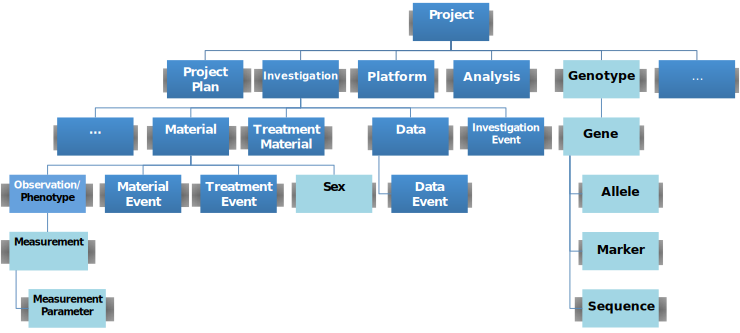
\includegraphics[trim = 0mm 30mm 0mm 48mm, clip,width=160mm]{podd_ont.pdf}
\vspace{-32pt}
\caption{Extended Domain Ontology for phenomics.}\label{fig:podd_ont}
\end{figure*}

\begin{itemize}
\item All essential concepts are modeled as subclasses of an abstract top-level OWL class \emph{PODDConcept} that captures common attributes and relationships.

\item All relationships between concepts are captured by domain properties, which can be further divided into two property hierarchies, one for parent-child relationships and the other for reference relationships. Each of the two hierarchies have an abstract top-level property, called \emph{contains} and \emph{refersTo}, respectively. 

\item All parent-child relationships are modeled in a property hierarchy as sub-properties of the abstract property \emph{contains}, and all reference relationships are modeled in another property hierarchy as sub-properties of the abstract property \emph{refersTo}.

\item For each domain concept $C$, one property is defined in each of the above hierarchies with its range defined to be $C$. The domains of such properties are not specified so that they can be used by any applicable domain concept to establish a relationship between them.

\item Class attributes are modeled using OWL restrictions.

\item Essential domain concepts can be sub-classed to provide more specialized and refined information. 

\item To ensure that each object can have at most one parent object, the inverse property of \emph{contains}, \emph{isContainedBy}, is defined so that a max cardinality restriction can be added to the top-level concept \emph{PODDConcept} to enforce it. 
\end{itemize}

The definitions of the top-level constructs are summarized in Figure~\ref{for:concept}, in OWL DL syntax~\cite{hoph03a}.

\vspace{-8pt}
\begin{figure}[htb]
\centering\small
\begin{zed}
PODDConcept \sqsubseteq \top\\
\top \sqsubseteq \forall contains.PODDConcept\\
isContainedBy \sqsubseteq (^-contains)\\
PODDConcept \sqsubseteq \leq 1~ isContainedBy\\
\top \sqsubseteq \forall refersTo PODDConcept
\end{zed}

\vspace{-12pt}
\caption{Top-level ontology constructs in the base ontology.}\label{for:concept}
\end{figure}

\vspace{-8pt}
\subsection{Roles of Domain Ontologies in Object Life Cycle}
The base ontology defines essential concepts independent of the domain. Domain-specific knowledge can be incorporated by extending the base ontology for discipline-specific systems.

As stated in Section~\ref{sec:intro}, the ontology-based domain model is at the center of the whole life cycle of objects. In this subsection, we briefly describe the roles that the domain ontologies perform at various stages of the object life cycle.

\begin{list}{\labelitemi}{\leftmargin=1em}
\item[\textbf{Ingestion}] When an object is created, its definition is expressed in ontological terms. Such definitions will be used to (a) guide the rendering of object creation interfaces and (b) validate the attributes and inter-object relationships the user has entered before the object is ingested. When an object is ingested, its definitions are stored as RDF assertions.

\item[\textbf{Retrieval \& update}] When an object is retrieved from the repository, its attributes and inter-object relationships are retrieved from its RDF assertions, which are used to drive on-screen rendering. When any value is updated, it is validated and updated in this object's RDF assertions.

\item[\textbf{Query \& search}] An object's assertions will be stored in an RDF triple store, which can be queried using the SPARQL query language~\cite{sparql}. Similarly, RDF assertions are indexed to provide functionalities such as full-text search and faceted browsing. 

\item[\textbf{Publication \& export}] When an object is published or exported, its metadata, in RDF, will be retrieved and exported.
\end{list}

\subsection{Integration with Existing Domain Ontologies}
As stated before, ontologies such as the Gene Ontology~\cite{citeulike:212874} and Plant Ontology~\cite{citeulike:3008167} are widely used in biomedical research to capture domain knowledge about genes, proteins, sequences and organism phenotypes. In our ontology-centric approach, these ontologies are used to extend our top-level ontology, add annotations on domain objects to enrich their semantic descriptions and enable cross-application reference and integration.

To describe domain knowledge in phenomics, we extend the base ontology by defining additional concepts including \emph{Genotype}, \emph{Gene}, \emph{Phenotype} and \emph{Sequence} as subclasses of \emph{PODDConcept}. Additional OWL object and datatype properties are also defined to model the attributes and relationships of these concepts, as shown in Figure~\ref{fig:podd_ont}. Note that \emph{Phenotype} is a subclass of \emph{Observation}. 

\section{The PODD Data Management System}\label{sec:sys}
\subsection{Implementation}
Based on the ontology-centric architecture presented in Section~\ref{sec:arch} and the base ontology presented in Section~\ref{sec:ont} we implemented the PODD data management system - with the aim being to meet the data management challenges faced by the Australian phenomics research community. 

In developing the PODD system, we chose to employ a number of mature technologies, as can be seen in Figure V. (1) We use Fedora Commons for the storage and retrieval of domain objects. Together with raw data files, the OWL (for concepts) and RDF (for objects) definitions of each concept and object are stored in a versioned datastream \texttt{PODD}, which is used by the PODD system in various tasks such as object creation, rendering, validation, update and visualization. Moreover, Fedora supports distributed storage through plugins, making it possible to increase the repository storage with demand. (2) We incorporate the Sesame\footnote{\url{http://www.openrdf.org/}} triple store to support complex query answering using SPARQL. Sesame \emph{contexts} are used to give scope to the RDF triples for each domain object. As described in Section III, access control needs to be enforced on a per project basis, which also needs to be enforced for query answering in the triple store. By identifying triples of individual objects, we are able to control contexts a user can access through query expansion. (3) We use the Solr\footnote{\url{http://lucene.apache.org/solr/}} open-source search engine platform to provide full-text search and faceted browsing capabilities. Similar to the structure of the Sesame triple store, there is a one-to-one correspondence between domain objects in the repository and the Solr \emph{documents}, the logical indexing units. (4) Lastly, we use a MySQL database to store user and access control related information, as it is orthogonal to other domain concepts.

\vspace{-8pt}
\begin{figure}[htb]
\centering
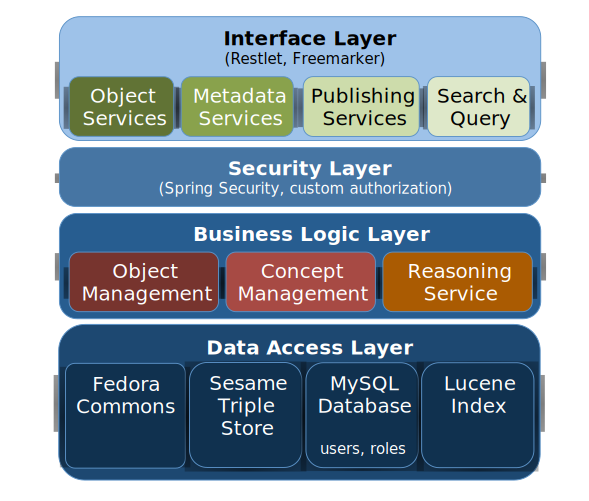
\includegraphics[trim = 60mm 30mm 50mm 24mm, clip,height=72mm]{podd_arch.pdf}

\vspace{-8pt} \caption{The architecture and main components of the PODD system.}\label{fig:podd_arch}
\end{figure}

\vspace{-8pt}
Although the architecture and the system are based on ontologies, the interface is designed to hide ontology-related complexity from the user and present information in an easy to use manner for all repository functions. For example, Figure~\ref{fig:browser} shows the browser view of a plant phenomics project that investigates salt tolerance in wheat breeding lines. In this view, the objects are shown in a tree-like structure by following parent-child assertions of subproperties of \emph{contains} defined in  the base and domain ontologies.

\begin{figure}[!t]
\centering
\includegraphics[trim = 0mm 0mm 0mm 0mm, clip,width=88mm]{browser.png}
\vspace{-16pt} \caption{The browser view of a plant project in the PODD repository.}\label{fig:browser}
\end{figure}

%\vspace{-8pt}
\subsection{Preliminary Evaluation}
We have started to deploy the PODD system in Australian phenomics research centers including APPF and APN and begun engaging users in the evaluation of the performance, flexibility, usability and scalability of the system. User feedback to date has shown that the system is intuitive and efficient.

It is well known that native RDF triple stores are not yet as efficient as relational database systems, especially in terms of query performance~\cite{10.1109/ICDE.2009.28,Bizer09theberlin}. In the PODD system, we employ a number of approaches to alleviate this problem. Firstly, we give scope to RDF triples of individual objects so a SPARQL query will only be matched against a (potentially very small) subset of the entire triple store, therefore improving query performance. Secondly, we index all RDF datatype property assertions and RDF type assertions in the Solr index to enable faceted searching and filtering. Together with the use of logical operators in search queries, full-text search can be used effectively to perform complex discovery tasks in most cases.

In summary, following the ontology-centric architecture and through the use of mature technologies, we have successfully developed PODD, a scalable, extensible data management system. At the same time, data management tasks such as versioning, logical organization of data, authentication \& authorization, and discovery, can all be supported effectively. The PODD system demonstrates the feasibility and practicality of the proposed ontology-centric architecture.

\section{Conclusion}\label{sec:concl}
In this work, our contribution to scientific data management is three-fold: firstly, the proposal of the ontology-centric architecture for developing highly extensible and domain-agnostic data management systems that supports the evolution of domain concepts; secondly, the development of a base ontology that defines essential concept in a domain-independent fashion; and thirdly, the development of a phenomics ontology and the data management system (based on both existing and new technologies) that serves as a validation of the feasibility of the proposed architecture. 

We have identified a number of future work directions that we would like to pursue. (1) We will investigate the integration with existing domain ontologies such as the Gene Ontology and the Plant Ontology. Potential approaches include using terms defined in these ontologies to annotate metadata objects, and establishing semantic links between concepts/properties through ontology alignment/mapping. (2) We would like to investigate the generalization of the ontology-centric approach and the further abstraction of the PODD base ontology so that the architecture can be applied to other domains including archeology, geological and environmental sciences. (3) Automated population of the PODD system of existing data can improve adoption of the system and alleviate the data entry burden for scientists. We have started working on developing tools for importing existing data in relational databases into PODD. (4) We will continue the development of the PODD system to provide additional functionalities such as data visualization, automated data integration, finer-grained representation of repository objects (file contents and metadata) in RDF, and Linked Data-style data discovery and publication. (5) Last but not least, we will investigate the feasibility of extending the PODD ontology and architecture to support scientific workflow modeling and composition.

\section*{Acknowledgment}
The authors wish to acknowledge the support of the National eResearch Architecture Taskforce (NeAT) and the Integrated Biological Sciences Steering Committee (IBSSC) Australia. The authors also wish to thank Dr. Xavier Sirault, Mr. Philip Wu and Dr. Kai Xu for the discussion and assistance in the development of the PODD ontologies and the PODD repository system.

\bibliography{all}
\bibliographystyle{IEEEtran}

\end{document}
